\subsection{Results}
\label{sec:mpi:results}

These results show the attained speedups for the MPI implementation.
Due to SeARCH limitations, only tests with two nodes were able to run (see \cref{sec:env, sec:method} for further details regarding the environmental setup and methodologies used, respectively).
Speedups are compared against the original sequential version in \cref{fig:mpi:results}.

\begin{figure}[!htp]
	\centering
	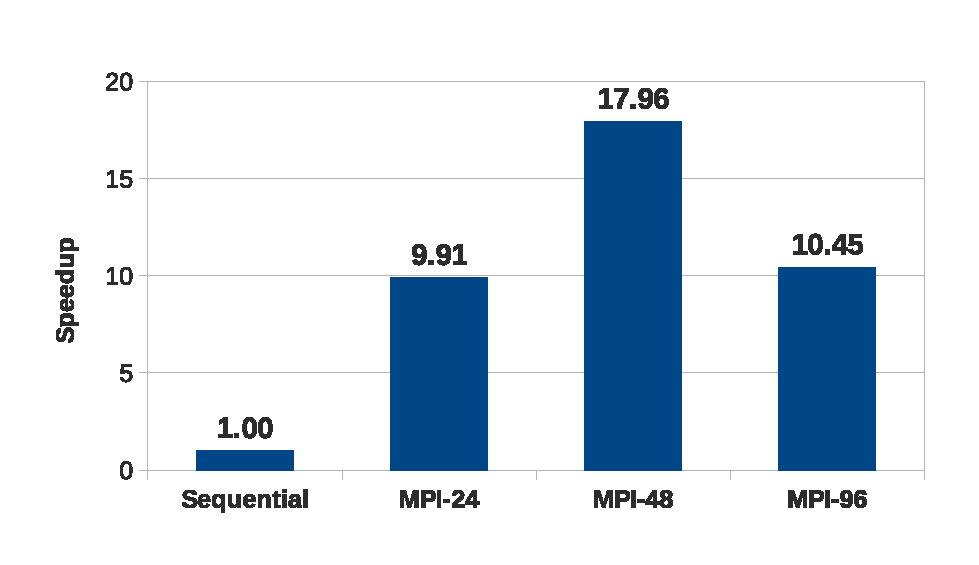
\includegraphics[width=\columnwidth]{graph_comparison_mpi}
	\caption{MPI implementation speedups.}
	\label{fig:mpi:results}
\end{figure}

While there are actual speedups, especially using 48 processes, the results are not as good as the shared memory results.
The reason for this comes from the nature of the algorithm, that makes it very sensible to the overhead of communications.
This imposes large limits to the scalability of any shared memory implementation of \polu.

\todonaps{Acho que aqui queres dizer distributed memory implementation, mas não mudei porque não percebo exactamente o que queres dizer com large limits.}
